\begin{frame}{Bottlenecks of (Jacobian-free) Newton-Krylov}
  \begin{columns}
    \begin{column}{0.4\textwidth}
      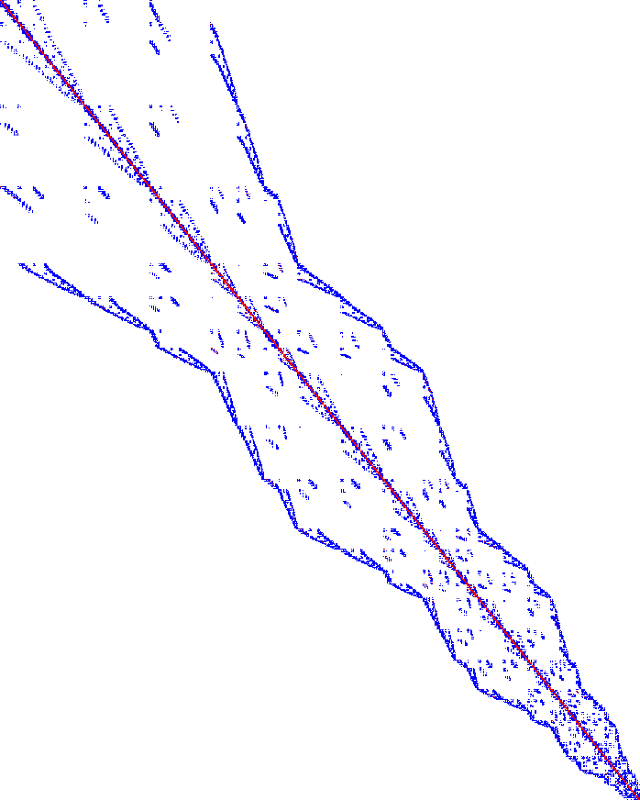
\includegraphics[width=1.15\textwidth]{figures/Dohp/EllipRCM}
    \end{column}
    \begin{column}{0.6\textwidth}
      \begin{itemize}
      \item Matrix assembly
        \begin{itemize}
        \item integration/fluxes: FPU
        \item insertion: memory/branching
        \end{itemize}
      \item Preconditioner setup
        \begin{itemize}
        \item coarse level operators
        \item overlapping subdomains
        \item (incomplete) factorization
        \end{itemize}
      \item Preconditioner application
        \begin{itemize}
        \item triangular solves/relaxation: memory
        \item coarse levels: network latency
        \end{itemize}
      \item Matrix multiplication
        \begin{itemize}
        \item Sparse storage: memory
        \item Matrix-free: FPU
        \end{itemize}
      \item Globalization
      \end{itemize}
    \end{column}
  \end{columns}
\end{frame}
